% PART 3
%\section{Model of de-identification process}
\section{Threat Model} \label{sec:threat-model}

For the purposes of threat modelling, the processes and actors involved in the creation and use of de-identified data are shown in \figref{fig:dfd}. While there are many threats that could potentially undermine the de-identification process (e.g. penetration of the club's computer systems, or manipulation of the pseudorandom number generator used to generate identifiers), the focus of this chapter is on threats to participant privacy due to inherent weaknesses in the de-identification methods themselves rather than attacks on the surrounding computational infrastructure (while attacks on the computational infrastructure are obviously an important concern in practice, these are not specific to the de-identification process).

%Threat model image
\begin{figure}[htbp]
  \centering
  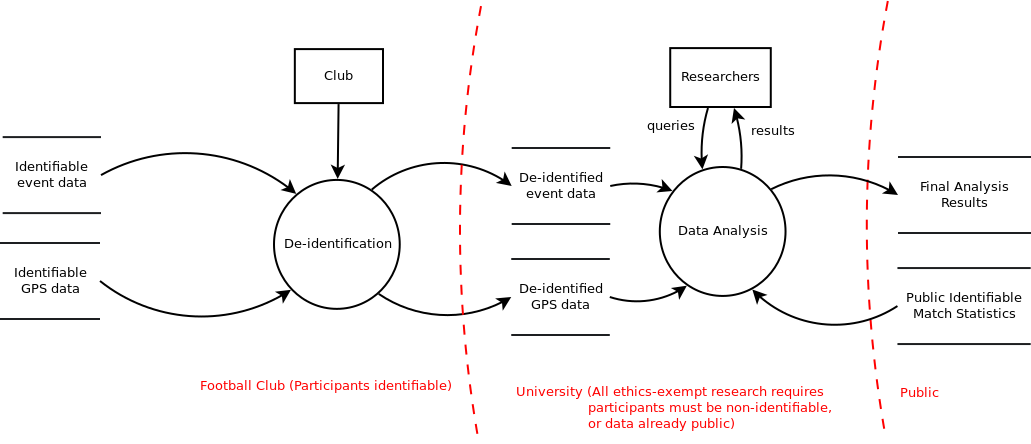
\includegraphics[width=\linewidth]{architecture-dfd}
  \caption{Data Flow Diagram for data de-identification, analysis, and publication. For purposes of threat modelling, trust boundaries (presented as red dashed lines) are marked to delineate the participant privacy protections that must be maintained within each organisation}
  \label{fig:dfd}
\end{figure}

% % TODO: Image showing data linkage within threat model
% \todo{Value of GPS Data}

%\subsection{Assets}

While AFL matches are played in public, and match statistics for each player and video footage are made publicly available, there are additional datasets the public do not have access to. This section provides a brief summary of these datasets, highlighting how they provide access to player information beyond what the public has access to. There is risk to players that if an attacker or unethical researcher were able to re-identity the dataset, it could cause discomfort to players through an unprecedented level of player scrutiny, or be used in ways contrary to the players' wishes, such as to inform betting odds.


% "VALIDITY AND INTERUNIT RELIABILITY OF 10 HZ AND 15 HZ GPS UNITS FOR ASSESSING ATHLETE MOVEMENT DEMANDS, Johnston et al. 2014"
% "At least one manufacturer has commenced supplementing 10 Hz GPS sampling with accelerometer data to provide in effect a 15 Hz sample rate" -- Applications of GPS Technologies to Field Sports, .Robert J Aughey
%  which would make it possible to recover accelerations from the augmented position tracking data even if the GPS units themselves are not well suited to capturing short term accelerations
% See Catapult Sports, ``Demystifying sample rate in satellite-based athlete tracking technologies'' \url{https://www.catapultsports.com/blog/sample-rate-satellite-athlete-tracking-technologies} Accessed: \dt{2019-11-25}
% \footnote{The IMU readings themselves provide valuable (and potentially sensitive) information for sport performance analysis. The de-identified tracking data in this thesis includes only position tracking data (latitude, longitude, time) rather than accelerations. However, some manufacturers use sensor fusion to combine information from IMUs with information from GPS units in order to provide higher frequency position estimates \cite{Aughey2011}. This would potentially make it possible to recover accelerations from the augmented position tracking data even if the GPS units themselves are not well suited to capturing short term accelerations. Note however that this does not necessarily lead to improved position accuracy. See Catapult Sports, ``Demystifying sample rate in satellite-based athlete tracking technologies'' \url{https://www.catapultsports.com/blog/sample-rate-satellite-athlete-tracking-technologies} Accessed: \dt{2019-11-25}}

% What do you call the leads on heart rate monitors? (Heart rate straps -- or if EEG, Electrodes)
Nowadays, all players wear position tracking devices on their back during each game. These devices are equipped with GPS units, in addition to Inertial Measurement Units (IMUs) containing accelerometers and gyroscopes that complement\footnote{Accelerations captured by IMUs can provide valuable \cite{Neville2010} (and potentially sensitive) insights into sport player performance, independent of the position tracking data. While IMU data are typically treated separately to GPS data, some manufacturers use sensor fusion to combine information from IMUs with information from GPS units in order to provide high frequency position estimates \cite{Aughey2011}. Note however, that higher frequency does not necessarily mean better accuracy. See Catapult Sports, ``Demystifying sample rate in satellite-based athlete tracking technologies'' \url{https://www.catapultsports.com/blog/sample-rate-satellite-athlete-tracking-technologies} Accessed: \dt{2019-11-25}} the GPS position estimates for short distances. The devices also have the ability to record heart rate; however, heart rate straps not always worn during games. Because the devices contain accelerometers, they are capable of detecting each footstep that a player makes. It has been suggested that accelerometers could be used to determine onset of musculoskeletal injuries by detecting asymmetries in acceleration between each foot \cite{Williamson2013}. Commercial sport position tracking device manufacturers have incorporated running symmetry analysis functionality into their software and claim that it can differentiate healthy players from those in rehabilitation.\footnote{GPSports, ``Running Symmetry Analysis,'' 2014. \url{https://web.archive.org/web/20140717135307/http://gpsports.com/running-symmetry-analysis/}} However, the validity of the running symmetry analysis reported by commercial devices has been questioned \cite{Kenneally-Dabrowski2018}. Nevertheless, the possibility that position tracking devices may reveal player injuries or other health conditions (albeit in its research infancy) highlights the importance of ensuring these data are properly de-identified before sharing them.

% https://www.sciencedirect.com/science/article/pii/S1877705811010307 "Evaluation of the use of a GPS data-logging device in a snowsport environment"
% states that "Heart rates are recorded to the SPI Elite using a wireless Polar T34 heart rate chest strap pickup"

% Possibly relevant: "Performance analysis of elite rugby league match play using global positioning systems", CP McLellan

% https://patents.google.com/patent/AU738702B3/en?q=gpsports&oq=+gpsports
% https://www.catapultsports.com/products/gpsports-evo?redirect=true&url=/faqs/Exertion_Scores.pdf "Polar compatible Heart Rate pickup
% T31 & H1 straps recommended"
% https://community.myfitnesspal.com/en/discussion/1286921/hrm-coded-vs-uncoded
% Seems that Polar heart rate strap wirelessly transmits data.

% however heart rate is usually not recorded during games as the ECG electrodes are uncomfortable (not certain about this statement)
% They can be used for determining player health information, such as determining if the player has a weak leg. The detail is apparent in \figref{fig:footsteps}, which clearly shows the profile of each footstep a player (or in this example, an AFL umpire) takes.

% Removed (only include ethics-approved material in thesis)
% \begin{figure}[ht]
%   \centering
%   \includegraphics[width=\linewidth]{umpire-footsteps}
%   \caption{Position tracking devices supplement GPS data with Inertial Measurement Sensors (IMU). The accelerometers are capable of detecting the profile of each footstep, as well as running asymmetries (e.g. due one leg being weaker than the other), which could reveal player injuries.}
%   \label{fig:footsteps}
% \end{figure}

% TODO: copy spiel about why AFLPA is concerned about leak of the player data.

Champion Data, the official AFL statistics provider, manually record each on-field event that occurs during the game, including the time at which it occurred. These are shared with teams as ``possession chain'' data, which can be used to scrutinise each action that a player makes. While one could theoretically derive the possession chain data via manually coding public match footage themselves, it would be prohibitively time consuming to code every match to the same level of quality that Champion Data provide. Thus while Champion Data possession chains for a short match segment do not provide any information beyond what is publicly accessible, when taken over a long period they may reveal highly detailed player profiles beyond that in the public domain.

When possession chain data and GPS data are de-identified using the same scheme such that the two datasets can be linked, it means that a compromise of the de-identification scheme used by \textit{either} of the datasets can be used to de-identify \textit{both} datasets via the data linkage. Analogous to the concept of privileged escalation in computer security, the concern is that re-identifying a player in a non-sensitive dataset such as short segment of possession chain information could lead to compromise of a more sensitive dataset, such as re-identifying player GPS traces for the length of the entire game which in turn could reveal sensitive knowledge about a player due to the fine-grained level that GPS devices can capture player movements when complemented with IMUs.

Attacks against possession chain data are demonstrated on a sample of possession chain data for one match during the 2015 season.\footnote{As noted, possession chains can be derived from public match footage. Thus privacy issues only arise when possession chain data are recorded over multiple matches in order to build detailed player profiles or linked to GPS data.} Attacks against GPS data are demonstrated by explaining how player trajectories could have been re-identified if it were not for the de-identification approach used in this thesis.

\section{Re-identification of Sport Data}
%\section{Attacks against common methods for de-identification of sport data}
\label{sec:de-identification-methods}

%\subsection{Methods to prevent re-identification of possession chain data}
\subsection{Re-identification of possession chain data}
\label{sec:de-identification-methods-possession-chain}

% Other angle: Public datasets, such as TV footage, may reveal heart rate.
% https://theconversation.com/protecting-your-privacy-if-you-use-a-route-mapping-app-58512

%\subsubsection{Method 1: Removal of date and venue}
\subsubsection{Attacks against removal of date and venue}
\label{sec:de-identification-methods-possession-chain-venue}

This section begins by outlining a simple attack to re-identify player possession chain data, an example of which is provided in Table \ref{tab:chains}. Possession chain data may also include the time of each event, but as will be shown, the events alone are enough to re-identify the players that perform them. In the example, the team and player fields have been anonymised through substitution of player names with anonymous identifiers. The example further attempts to thwart the attacker by removing all details about the match, and assumes the attacker only knows minimal details such as that it was an AFL match occurring on an unknown date at an unknown time during the main 2015 season.

% \nb{Thought: Note the parallels between de-identification by replacing names with anonymous identifiers, and a simple substitution cipher (which is obviously not secure!). Perhaps we can take lessons from cryptography to reason about the strengths/weaknesses of de-identification schemes.}

% Generated by http://www.tablesgenerator.com/
\begin{table}[h]
\centering
\caption{``Anonymised'' Player Scoring Chain Data}
\label{tab:chains}
\begin{tabular}{llllll}
Chain & Team & Chain Start Type & Chain End Type & Disposal & Player ID \\
1     & B    & Stoppage - CB    & Rushed         & kick     & 131                  \\
2     & A    & Kick In          & Stoppage - TU  & kick     & 123                  \\
3     & B    & Stoppage - TU    & Stoppage - TI  & kick     & 108                  \\
4     & B    & Stoppage - TU    & Goal           & kick     & 137                  \\
5     & A    & Stoppage - CB    & Turnover       & kick     & 124                  \\
6     & B    & Turnover         & Turnover       & kick     & 104                  \\
7     & A    & Turnover         & Goal           & kick     & 139                  \\
7     & A    & Turnover         & Goal           & handball & 126                  \\
7     & A    & Turnover         & Goal           & kick     & 122                  \\
8     & B    & Stoppage - CB    & Turnover       & kick     & 117
\end{tabular}
\end{table}

% An attacker can trivially re-identify the players through the frequency of each action in order to create a fingerprint that can be compared to public player statistics.

An attacker can use the frequency of each action players perform as a fingerprint that the attacker can compare to public player statics to re-identify players. An attacker does not require any specialised skills or software to do this; indeed, an attacker can perform this task in a matter of seconds using an Excel pivot table, as shown in \figref{fig:pivot}.

\begin{figure}[h]
  \centering
  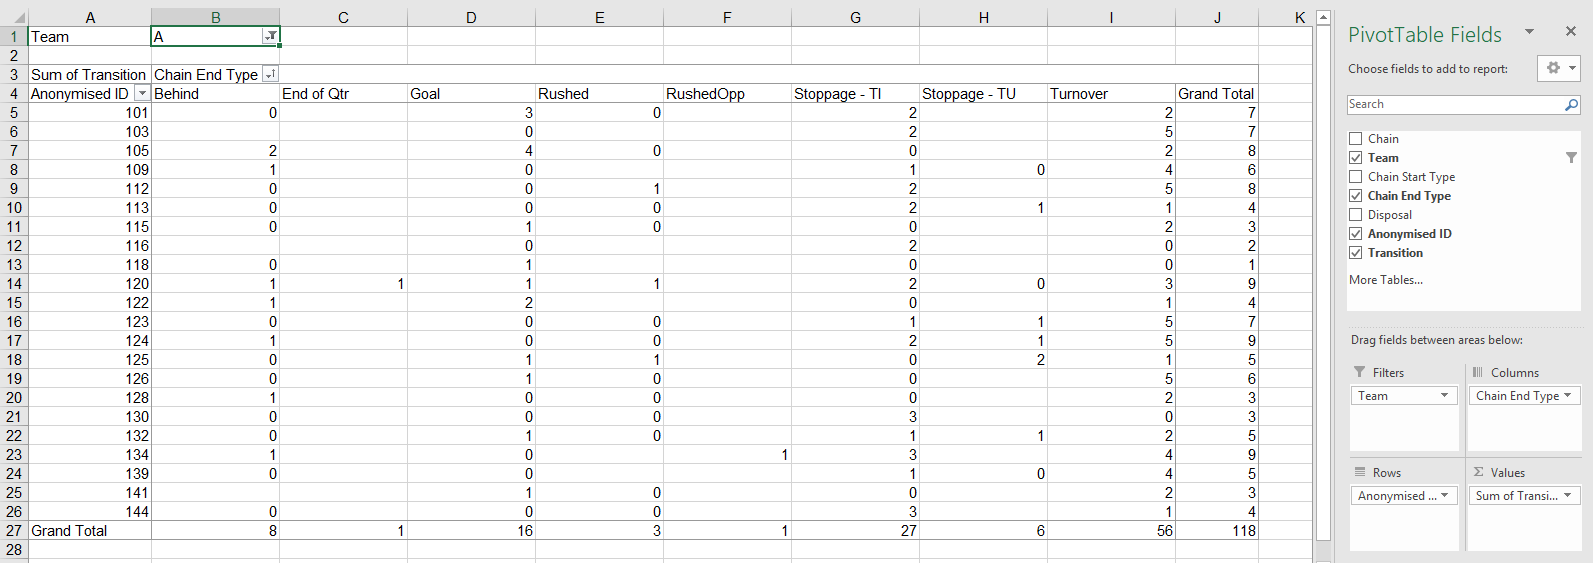
\includegraphics[width=\linewidth]{pivot-table-deidentification-scrshot}
  \caption{Given scoring chain data, an attacker can easily tabulate summary statistics at both a team and player level in a matter of seconds using an Excel pivot table}
  \label{fig:pivot}
\end{figure}

The tabulation (\figref{fig:pivot}) reveals that team A scored a total of 16 goals, and 11 behinds (8 ordinary behinds, 3 ``rushed'' behinds). This is typically reported as "16.11". The attacker then consults a table of matches played during the season, such as that found at AFL Tables\footnote{\url{https://afltables.com/afl/seas/2015.html}}, and searches for text "16.11". In 2015, there was only one team that scored this exact combination of goals and behinds: Hawthorn in the 2015 grand final. This shows that removing the date of match and team names did not serve as any meaningful guard of participant privacy, as an attacker was able to infer this information through using the score totals as a fingerprint.
% using a na\"{\i}ve search space reduction strategy.
% was originally "with negligible effort", but supervisor suggested change to "using a naive search space reduction strategy"

\subsubsection{Attacks against substitution of participant identifiers in event data}

Once the attacker obtains the match information, they can proceed to re-identify individual players. A player's actions serve as a fingerprint. For example, the tabulation (\figref{fig:pivot}) shows that player 105 (row 7) scored 2 behinds and 4 goals. The attacker can compare this with the public player statistics for that game\footnote{\url{http://www.afl.com.au/match-centre/2015/27/haw-v-wce}}, which uniquely identifies this player as Cyril Rioli. Now that the attacker knows Cyril Rioli = player 105, they can scrutinise this player's full scoring chain data as well as any other datasets that were de-identified using the same player code.

%\subsection{Methods to prevent re-identification of GPS data}
\subsection{Re-identification of GPS data}
\label{sec:de-identification-methods-gps}

%\subsubsection{Method 3: Substitution of participant identifiers in spatio-temporal data}
\subsubsection{Attack against substitution of participant identifiers in spatio-temporal data}

As explained in \secref{sec:deidentification-of-spatial-data}, spatio-temporal data are inherently difficult to de-identify. GPS devices record both player location, and precise time. Even a single time-instant is enough for the attacker to re-identify which traces belong to which players via comparison to match video footage---for example, in \figref{fig:vid}, an attacker re-identifies the players involved in the \centrebounce{} at the start of the 3rd quarter, a task that is made easy by the large numbers printed on players' guernseys to make their identity known. Once the attacker has re-identified a player at one time instant, they can examine the minute details of every movement a player makes over the course of the match, including the profile of each footstep.

\begin{figure}[htbp]
  \centering
  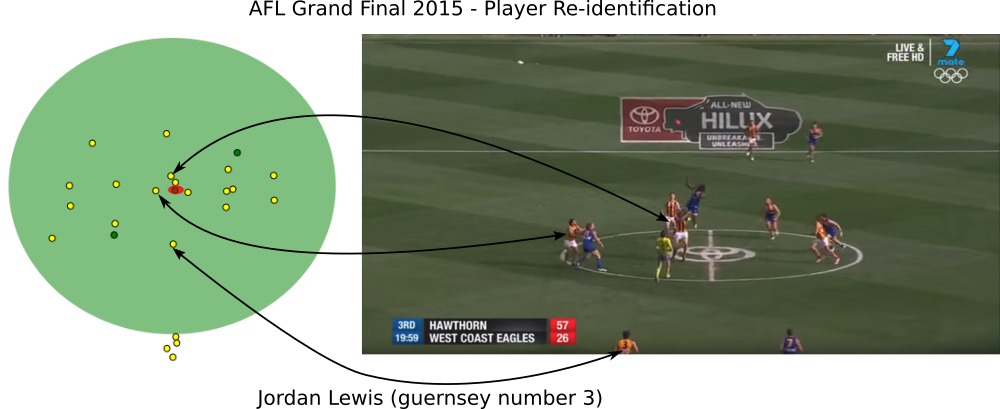
\includegraphics[width=\textwidth]{grand-final-2015-player-reidentification}
  \caption{Left: Location of players on field at start of 3rd quarter, as obtained from GPS data. Right: Video footage of game 1 second into the 3rd quarter. Given ``anonymised'' GPS data, an attacker can easily re-identify players through comparison with video footage}
  \label{fig:vid}
\end{figure}

%\subsubsection{Method 4: Spatio-temporal distortions}
\subsubsection{Attacks against spatio-temporal distortions}

\begin{figure}[htbp]
  \centering
  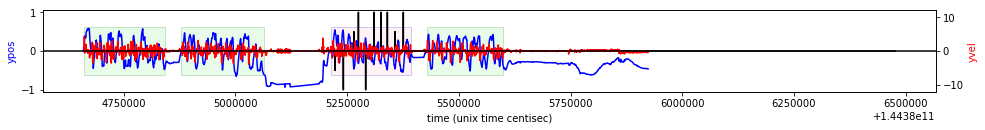
\includegraphics[width=\textwidth]{gps-time-sync-t}
  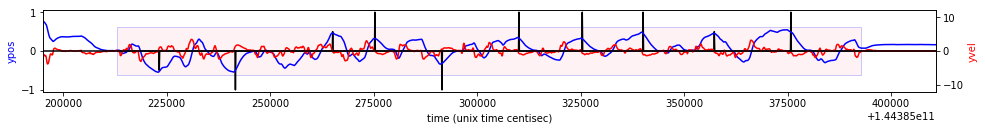
\includegraphics[width=\textwidth]{gps-time-sync-b}
  \caption{Top: Average position in direction of goals (blue line) and velocity (red line) of players during match, as obtained from GPS data. The overlaid rectangles show the duration of each quarter, which correspond with the level of activity. Bottom: A zoomed in section of the above focusing on the third quarter. The overlaid vertical black bars represent the time of goals (large bar) and behinds (short bar) for each team (direction of bar). Note that the time of goals and behinds correspond to peaks and troughs of average team position (blue line) in the direction of goals, and short periods of inactivity (red line crossing x-axis) after a goal is scored.}
  \label{fig:gps-time-sync}
\end{figure}

% Futility of time distortion.
One could attempt to prevent the ability of the attacker to re-identify the GPS data by shifting and/or distorting the time axis. However, this is unlikely to offer any meaningful protection, as events in the GPS data align closely with scoring events (see \figref{fig:gps-time-sync}), thus allowing the attacker to re-identify the precise game instants that the GPS data correspond to. Indeed, in the datasets used in this thesis, the precise time of match events were not provided; however, in most cases\footnote{In quarters where teams scored periodically at consistent time intervals, offsets of $n\cdot {interval\ duration}$ provided a good fit for any $n$, and thus automatic time synchronisation sometimes selected the wrong offset in these edge cases. These cases were identified and resolved through manually inspecting the GPS formations at key events and interactively manipulating the time offset to find a better fit (\secref{sec:integration-timesync}). As these edge cases could be corrected manually, it is likely that a fully automated approach may be possible using a more sophisticated algorithm that examines the entire team formation rather than just average team position and velocity.} it was possible to automatically synchronise these with the GPS data through optimising for the time shift that resulted in the best alignment of match events with peaks and troughs in the GPS data. One could attempt to counter this through non-uniform time distortions; however, this would risk compromising the quality of the analysis due to distortion of player speed, and could still be circumvented through the use of a more sophisticated temporal comparison algorithm, such as Dynamic Time Warping (DTW).

% Supervisor requested that the image be near the text to improve readability (thus preventing the examiners from flipping between pages)
\begin{figure}[!htb]
  \centering
  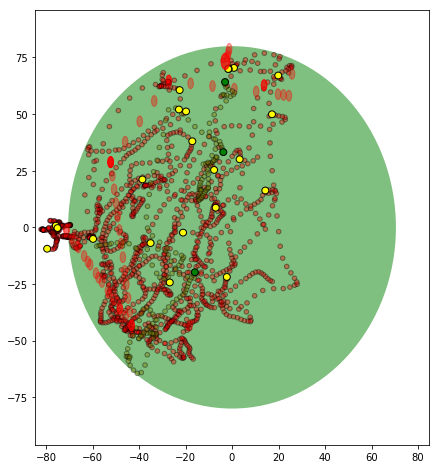
\includegraphics[width=0.5\textwidth]{gps-r27-q3-t622}
  \caption{1 minute of player GPS movements during a game, as the ball is passed along the edge of the field. The true shape of the field is indicated by the green oval; however, the location of the interchange area (left of image) and shape of the oval are visually apparent from the GPS data alone.}
  \label{fig:gps-edge-field}
\end{figure}

% Futility of direction distortion
One may also attempt to prevent the ability of the attacker to re-identify the GPS data by performing spatial translations, rotations, and reflections. However, players frequently pass the ball along the edge of the field, which makes the bounds of the field visually apparent; an example of GPS movements that reveals the edge of the field is shown in \figref{fig:gps-edge-field}. Once the shape of the field is identified, the only additional details that an attacker need to concern themselves with are identifying any reflections. However, this can be achieved by examining the GPS data at the time of a goal to see which side of the field the players were occupying. Indeed, in the datasets used in this thesis, none of the datasets included the ``coin-toss'' used to decide which direction players goals are; however, it was still possible to infer this through considering both possible directions then choosing the direction that resulted in the best alignment with the public match event feed. In conclusion, linear spatial transformations are insufficient to prevent player re-identification. Any operation that distorts scale, including non-homogeneous scale distortions such as a non-linear transformation, are not an option, as they would affect most forms of spatial analysis such as player speed. Furthermore, the attacker can use known information about a player's typical speed to infer the scale distortion, thus allowing the transformation to be inverted.

%\subsubsection{Method 5: Complete removal of identifiers}
\subsubsection{Preventing attack by complete removal of identifiers}
\label{sec:de-identification-removal}
% Complete removal of identifiers

% Supervisor: {Should proposals come as part of the framework?}
% thought: could make logic of attacks and counter-attacks clearer by using CORAS diagram

Due to the ease with which an attacker can undermine the aforementioned de-identification methods, it is necessary to consider a more extreme approach. Note that the value to an attacker lies in the ability to re-identify players at one time instant, and then use this to re-identify the player at other time instants, or in the case of linked datasets, to re-identify the player in other datasets that use the same anonymised player code. By completely removing the player identity column, the link between player movements at different time-instants can be destroyed.

An example of a fully de-identified possession chain data is given in Table~\ref{tab:chains-v2}. The team name is not anonymised in the example, because as previously shown, teams can be trivially re-identified by an attacker based on the number of scoring events\footnote{An attack to re-identify the team name is covered in \textit{Attacks against removal of date and venue} (\secref{sec:de-identification-methods-possession-chain-venue})} yet removing team names would hinder legitimate data analysis seeking to compare identified patterns to public information about the team.
% As sets are invariant to permutations, the order of player locations in the serialised data can be shuffled.

% Generated by http://www.tablesgenerator.com/
\begin{table}[htbp]
\centering
\caption{Player Scoring Chain Data, de-identified by completely removing player identifiers}% in accordance with Sec.~\ref{sec:de-identification-removal}}
\label{tab:chains-v2}
\begin{tabular}{llllll}
Chain & Team & Chain Start Type & Chain End Type & Disposal & Player ID \\
1     & WCE  & Stoppage - CB    & Rushed         & kick     & NULL      \\
2     & HAW  & Kick In          & Stoppage - TU  & kick     & NULL      \\
3     & WCE  & Stoppage - TU    & Stoppage - TI  & kick     & NULL      \\
4     & WCE  & Stoppage - TU    & Goal           & kick     & NULL      \\
5     & HAW  & Stoppage - CB    & Turnover       & kick     & NULL      \\
6     & WCE  & Turnover         & Turnover       & kick     & NULL      \\
7     & HAW  & Turnover         & Goal           & kick     & NULL      \\
7     & HAW  & Turnover         & Goal           & handball & NULL      \\
7     & HAW  & Turnover         & Goal           & kick     & NULL      \\
8     & WCE  & Stoppage - CB    & Turnover       & kick     & NULL      \\
\end{tabular}
\end{table}

Position tracking data are typically stored as separate files for each individual player trajectory. Even if the files names contain no identifying information, storing a single player's trajectory for the entire match in the same file means that the player can be re-identified for the duration of the entire match if an attacker can re-identify the player at a particular moment. For example, if an attacker knows that a particular player scored a goal at a particular time, they can re-identify the trajectory file for that player by searching for trajectory files that contain a point at that time and location. This then gives the attacker access to detailed movements of that player over the course of the entire match.

This can be prevented by merging all the player traces together and splitting them into a sequence of team formations at each time instant. Representing the team formation as a \textit{point cloud} (an unordered set of points) removes the link between player locations at different time instants. While this prevents individual player analysis, it still permits many forms of team analysis methods. %, such as \textit{point pattern analysis} (analysis methods that operate on point clouds). (point pattern analysis seems to be more to deal with repeating patterns, e.g. tree locations)
A visual explanation is provided in \figref{fig:pointcloud}. This approach was inspired by Ding et al. \cite{Ding2017} who show that randomly mixing human trajectories whenever two people cross paths prevents re-identification of individuals, while still allowing certain forms of analysis about the group.

% Similarly, position tracking data can be represented point cloud
% while this prevents individual player analysis, it still permits many forms of team analysis methods, such as point pattern analysis.

\begin{figure}
  %\includegraphics{/path/to/figure}
  \centering
  $Formation = \{(x_a, y_a), (x_b, y_b), ...\} = \{(x_b, y_b), (x_a, y_a), ...\}$
  \caption{A point cloud is an unordered set of points. Representing team formations in this manner allows analysis of the team, while removing ties to individual player identities. As operations on sets are invariant to the ordering of elements within the set, the ordering of players within the formation can be randomised when serialising the data to deter attackers without affecting the analysis.}
  \label{fig:pointcloud}
\end{figure}

% Supervisor: {can/could is mixed in text. Aim for ``can'' as it will be easier to read as an active sentence.} %(fixed)

To circumvent this method, an attacker can attempt to reconnect the links between locations belonging to the same player by pairing an occupied location at one instant with the closest occupied location the next time-instant. A more sophisticated approach can use player velocity to estimate the next location, then take the nearest occupied location to the estimated location. However, this would be difficult in practice as players often come into close contact with each other. Every time players interact, there is a branching of the possible locations the player could be in next. Thus while one can infer related player movements for a short period of time, the number of possible combinations increases with time \cite{Ding2017}. This means that even if an attacker were to determine a player's location at a certain point in time (e.g. from a photo at a known time instant), they will only be able to trace the player for a short time due to increasing uncertainty about which player is which when trying to trace players over the medium to long-term course of a match.

% Down-sampling?
\subsubsection{Downsampling}

As noted, the key threat to participant privacy is that an attacker can gain access to high frequency GPS data, that when complemented with accelerometers, can be used to track a player's individual footsteps, and thus potentially infer sensitive player information.\footnote{As outlined in \textit{Threat model} \secref{sec:threat-model}} While downsampling doesn't intrinsically serve as a de-identification technique, hence it will not be classified as a de-identification method in \secref{sec:trade-off}, lossy downsampling could result in a reduction of the sensitivity of player data, thus reducing the potential harm to participants if re-identified. It could also be used in combination with removal of identifiers to make re-identification via trace reconstruction harder, due to increased uncertainty of player movements when sampled at a lower frequency.

\section{Analysis of Trade-Off between Participant Privacy and Data Quality}
\label{sec:trade-off}

This section compares the strength of each de-identification method outlined in \secref{sec:de-identification-methods}, and considers how the de-identification impacts on the utility of the data to researchers. Specifically, it considers the constraints on the kinds of analysis that can be performed as a result of de-identification of the data. This is presented in Table~\ref{tab:trade-off}.

% https://tex.stackexchange.com/questions/4139/how-to-change-font-size-mid-document/384163#384163

% Supervisor: {Formatting (do last)}

% repo: afl-player-deidentification
% https://www.tablesgenerator.com/
\begin{table}[h]
\centering
\caption{Analysis of trade-off between de-identification strength versus utility of data after de-identification}
\footnotesize % https://en.wikibooks.org/wiki/LaTeX/Fonts#Sizing_text
\hyphenpenalty=10000 % https://tex.stackexchange.com/questions/5036/how-to-prevent-latex-from-hyphenating-the-entire-document
\label{tab:trade-off}
\begin{tabular}{L{1.5cm}L{2.5cm}L{2.1cm}L{2.5cm}L{1.5cm}L{1.8cm}}
\specialcellb{\textbf{Data} \\ \textbf{Type} \\  \\\hspace{0pt}}        & \specialcellb{\textbf{De-}\\\textbf{identification}\\ \textbf{Method} \\\hspace{0pt}}                                       & \specialcellb{\textbf{Attacks}\\  \\  \\\hspace{0pt}}                              & \specialcellb{\textbf{Identifiable}\\\textbf{Data}\\ \textbf{Required}\\ \textbf{for Attack}} & \specialcellb{\textbf{Attack}\\ \textbf{Difficulty}\\ \\\hspace{0pt}} & \specialcellb{\textbf{Analysis}\\ \textbf{Constraints*}\\ \\\hspace{0pt}}                     \\
\hline
\rule{0pt}{4ex} % https://tex.stackexchange.com/questions/50352/inserting-a-small-vertical-space-in-a-table
Event Sequence   & Remove date and venue                                   & Fingerprint total events             & Totals of each event type                        & Low & Independent of date and venue                                    \\
\rule{0pt}{4ex} % https://tex.stackexchange.com/questions/50352/inserting-a-small-vertical-space-in-a-table
Event Sequence   & Substitute participant names with anonymous identifiers & Fingerprint total participant events & Totals of each event type for each participant   & Low &                                                                  \\
\rule{0pt}{4ex} % https://tex.stackexchange.com/questions/50352/inserting-a-small-vertical-space-in-a-table
Spatio- Temporal & Substitute participant names with anonymous identifier  & Compare to video or images                     & Photograph of participants at known time instant & Low &                                                                  \\
\rule{0pt}{4ex} % https://tex.stackexchange.com/questions/50352/inserting-a-small-vertical-space-in-a-table
Spatio- Temporal & Spatio-temporal distortions                             & Correlate with event sequence        & Sequence of key events                           & Medium & Invariant to translation, rotation, and reflection            \\
\rule{0pt}{4ex} % https://tex.stackexchange.com/questions/50352/inserting-a-small-vertical-space-in-a-table
Spatio- Temporal & Remove participant ids                                  & Reconstruct traces                   & Photograph of participants at known time instant & High & Invariant to participant permutations              
\end{tabular}

\vspace{1em}

* Additional analysis constraint for all de-identification methods:\\
Can only link to datasets that use same anonymous identifiers
\end{table}

%\section{De-identification strategy selection}

Attempts to prevent player re-identification, through replacement of names with anonymous identifiers, removal of event timestamps, and shifting/distortion time and space, are weak. An attacker can obtain data fingerprints for one or more players, and find the mapping between anonymised player code(s) and the player's identity.

The only method that offered protection against re-identification of players was complete removal of participant identifiers and use of a point cloud data structure (i.e. an unordered set of points) at each time-instant. This de-identification method removes the ability to trace the path of individual players. For stronger protection, this can be combined with downsampling of the position tracking data (e.g. from 10 Hz to 1 Hz\footnote{The sampling rate chosen depends on the application. Lower sampling rates offer stronger privacy, but discard information that may be needed for the analysis. The rate of 1 Hz was chosen for this thesis in order to match the needs of the analysis performed in \chref{ch:integration}, which analysed team-level formations at 1 second intervals. A higher sampling rate could have been chosen if the analysis required detailed player movements (at the cost of increased risk of data re-identification).}), thus increasing the uncertainty of player identities when two players come into close contact during the time window. This also has the effect of filtering out the high frequency component of the player position information that risks revealing individual player steps.

Note that in order to achieve privacy, it is necessary to reduce data quality, thus limiting the types of analysis that can be performed. However, if the goal is macro-level team-level analysis rather than micro-level studies of player movement, then this trade-off may be acceptable. Allowing individual player movements to be traced over the course of the match is in contradiction to the goal of de-identifying data; if individual player movements can be traced, then players can be fingerprinted by their movement and scoring patterns, and thus the dataset would be re-identifiable rather than non-identifiable.
